\chapter{视图}
\section{视图}
Django 的视图是一个 Python 函数，它接受一个 Web 请求并返回一个 Web 响应。
Django 的视图可以以多种方式编写，最简单的方式是作为一个函数。

\section{视图函数}
\subsection{视图函数——HttpResponse}
视图函数是Django中的一个重要概念，它是一个Python函数，接收一个Web请求(\codeinline{request})并返回一个Web响应(\codeinline{HttpResponse})。
视图函数的定义如下：
\begin{lstlisting}[style=demostyle, numbers=none]
def my_view(request):
    # 业务逻辑
    return HttpResponse('Hello, World!')
\end{lstlisting}   

\subsection{渲染模板——render}
\begin{lstlisting}[style=demostyle, numbers=none]
render(request, '模板名称', {'参数1': '值1', '参数2': '值2'})    
\end{lstlisting}

\begin{enumerate}[label=\arabic*)]
    \item 在项目的根目录下创建一个\codeinline{templates}文件夹，用于存放模板文件。
    \item 在\codeinline{templates}文件夹下创建一个与子应用同名的文件夹\codeinline{TestModel}，
    用于存放子应用\codeinline{TestModel}的模板文件。

    \item 在\codeinline{TestModel}文件夹下创建一个\codeinline{test.html}文件，用于存放模板文件。
    \item 在主项目的\codeinline{settings.py}中配置模板路径。
\begin{lstlisting}[style=demostyle, numbers=none]    
$> cat mysite/settings.py
...
BASE_DIR = os.path.dirname(os.path.dirname(os.path.abspath(__file__)))
...
TEMPLATES = [
    {
        'BACKEND': 'django.template.backends.django.DjangoTemplates',
        # 'DIRS': [],
        'DIRS': [os.path.join(BASE_DIR, 'templates')], # 指定模板文件的目录
        'APP_DIRS': True,
        ...
    },
]
...
\end{lstlisting}    
    \item 在子应用目录下的\codeinline{urls.py}中，修改\codeinline{test\_view}函数，使用\codeinline{render}函数渲染模板。
\begin{lstlisting}[style=demostyle, numbers=none]
from django.urls import path
from .views import test_view, test_index

urlpatterns = [
    path('test/', test_view),
    path('index/', test_index),
]
\end{lstlisting}    
    \item 在子应用目录下\codeinline{views.py}中定义\codeinline{test\_index}函数，使用\codeinline{render}函数渲染模板。
\begin{lstlisting}[style=demostyle, numbers=none]
from django.shortcuts import render
from django.http import HttpResponse

# Create your views here.
def test_view(request):
    return HttpResponse('Hello, Django!') # 返回一个字符串

# 渲染模板 —— render

def test_index(request):
    return render(request, 'TestModel/index.html') # 渲染index.html模板
\end{lstlisting}    
    \item 在浏览器中输入\codeinline{http://localhost:8000/index/}，即可看到如图\ref{fig:Django渲染html的过程}所示页面。    
\end{enumerate}


\begin{figure}[htpb]
    \centering
    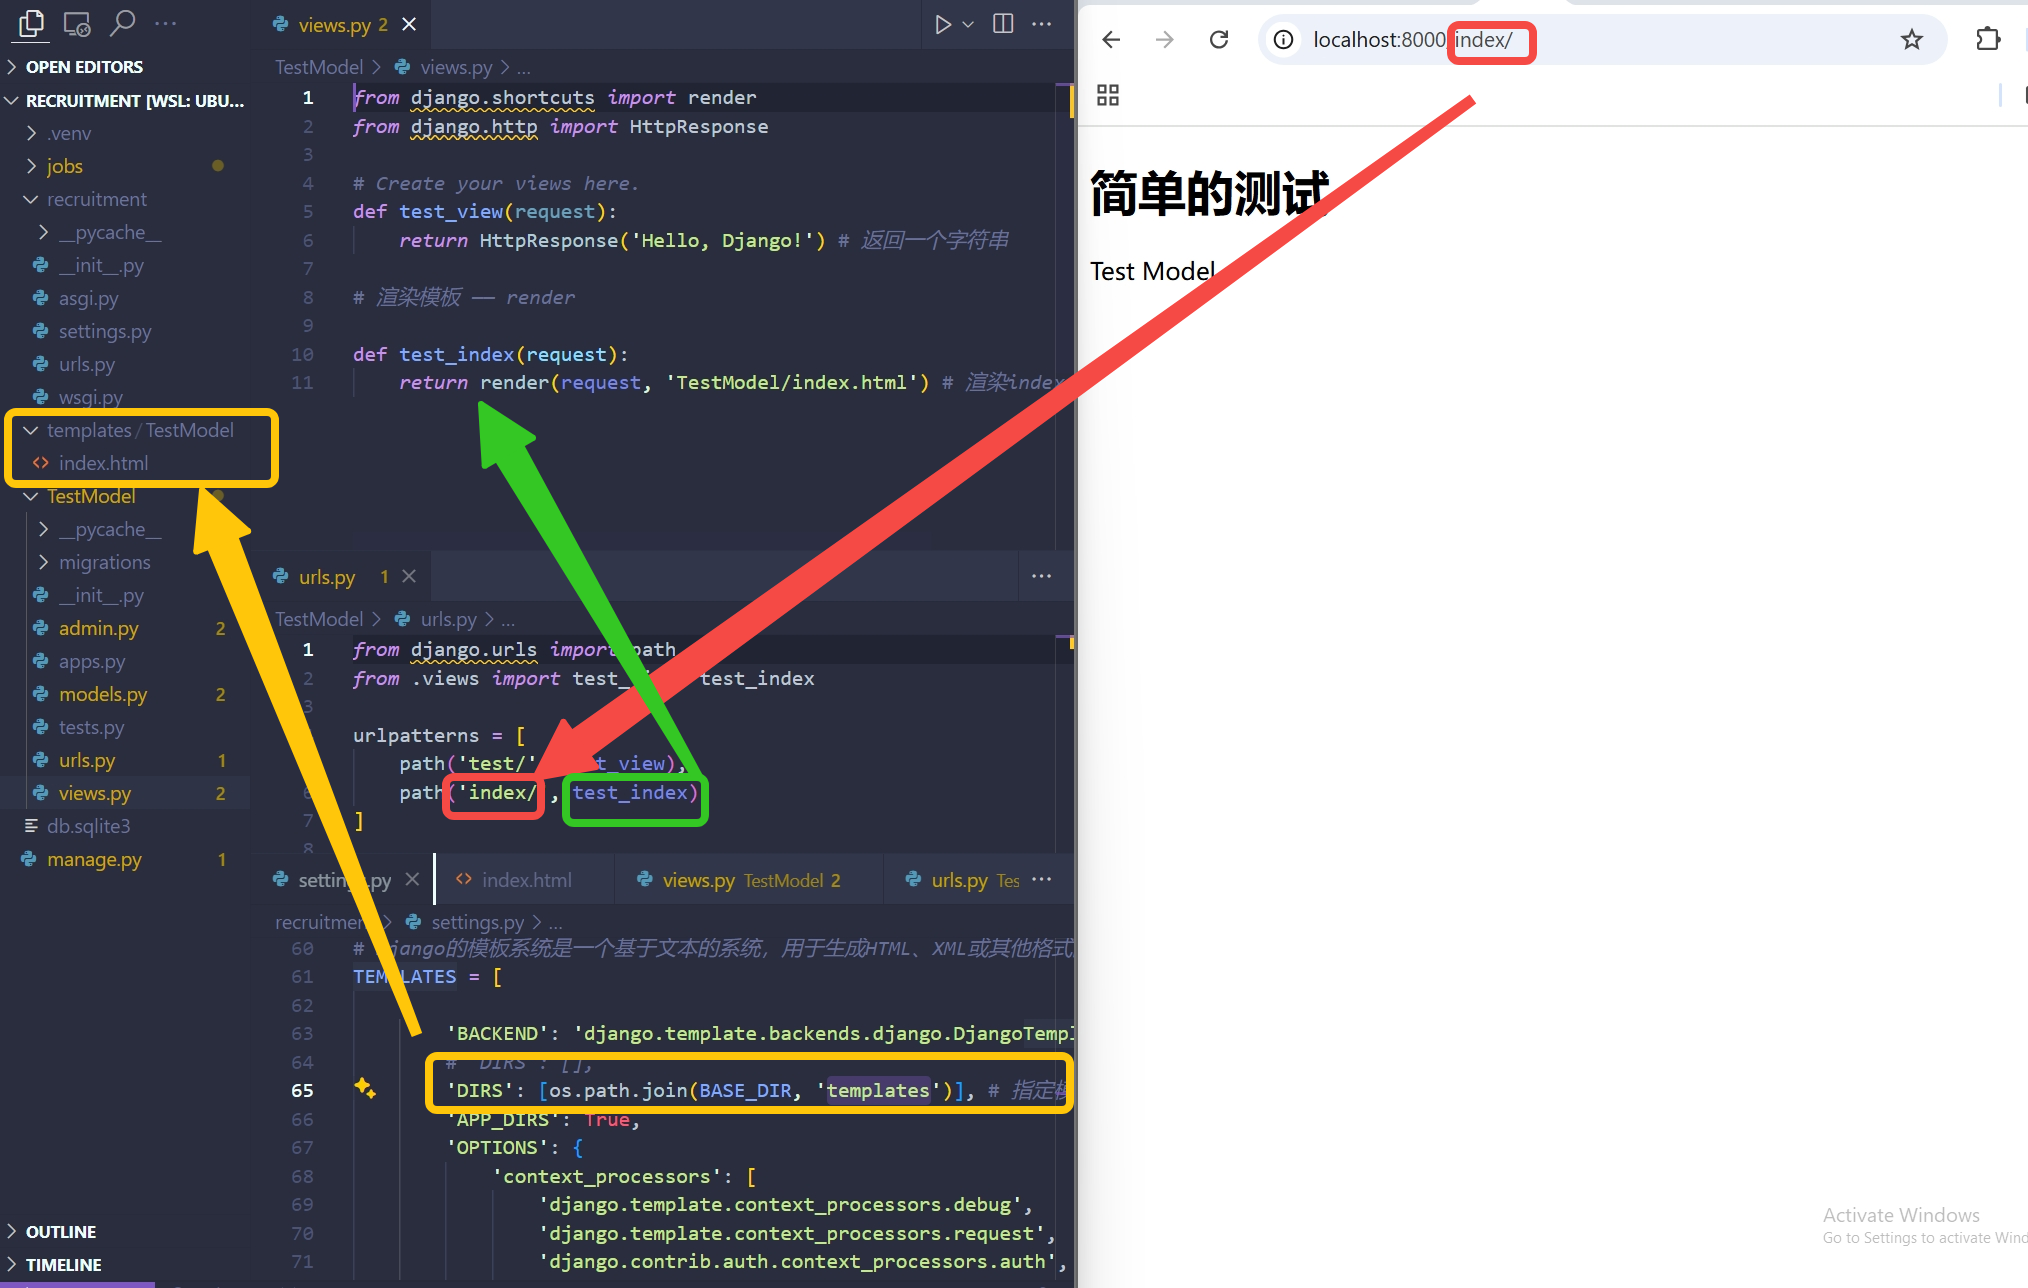
\includegraphics[width=0.6\textwidth]{part/互联/django/pic/视图/渲染html的过程.png}
    \caption{渲染html的过程}
    \label{fig:Django渲染html的过程}
\end{figure}

\section{URL配置(URLconf)}
URLconf 是 Django 中的 URL 配置，它是 URL 模式（URL 模式是 URL 和 Python 回调函数的映射）的集合。

一般在 \textcolor{YBXPurple}{主项目}目录下的\codeinline{urls.py}文件中配置 URLconf，用于将 URL 映射到 \textcolor{YBXPurple}{视图函数} 或 \codeinline{include}\textcolor{YBXPurple}{子应用}的 URLconf。

一般的格式为
\begin{enumerate}[label=\arabic*)]
    \item 主项目的\codeinline{urls.py}文件中，导入\codeinline{include}函数和子应用的\codeinline{urls.py}文件。
\begin{lstlisting}[style=demostyle,numbers=none]
from django.urls import path, include

urlpatterns = [
    # 直接引入视图函数
    path('路由名/', views.视图函数名),
    path('路由名/', views.视图函数名, name='视图函数名'),
    url(r'^路由名/', include('子应用.urls')),
    re_path(r'^路由名/', include('子应用.urls')),

    # 引入子应用的 URLconf
    path('子应用名/', include('子应用.urls')),
    url(r'^路由名/', include('子应用.urls')),
    re_path(r'^路由名/', include('子应用.urls')),
]
\end{lstlisting}
    
    \item 子应用的\codeinline{urls.py}文件中，导入视图函数。

\begin{lstlisting}[style=demostyle,numbers=none]
from django.urls import path, include
# 如果子应用有下面的一行，表示引入应用的 views.py 文件
from . import views    

urlpatterns = [
    path('路由名/', views.视图函数名),
    path('路由名/', views.视图函数名, name='视图函数名'),
]
\end{lstlisting}    
\end{enumerate}

\subsection{path() 将URL模式映射到视图}
\codeinline{path()}函数用于将 URL 模式映射到视图。

它采用四个参数，两个必选参数：route 和 view，两个可选参数：kwargs 和 name。
\begin{lstlisting}[style=demostyle,numbers=none]
from django.urls import path

path(route, view, kwargs=None, name=None)
\end{lstlisting}  
\begin{enumerate}[label=\arabic*)]
  \item \codeinline{route}: 字符串，定义 URL 的路径部分。
  
  可以包含变量，例如 \codeinline{<int:my\_variable>}，以从 URL 中捕获参数并将其传递给视图函数。

  \item \codeinline{view}: 视图函数，处理与给定路由匹配的请求。
  
  可以是一个函数或一个基于类的视图。
  
  \item \codeinline{kwargs}(可选): 一个字典，包含传递给视图函数的额外关键字参数。
  
  \item \codeinline{name}(可选): 为 URL 路由指定一个唯一的名称，以便在代码的其他地方引用它。这对于在模板中生成 URL 或在代码中进行重定向等操作非常有用。
\end{enumerate}

\subsection{[弃用] url()/re\_path 将URL模式映射到视图}
\codeinline{url()}函数用于将 URL 模式映射到视图。
\begin{lstlisting}[style=demostyle,numbers=none]
from django.urls import include, url

url(regex, view, kwargs=None, name=None, prefix=None)
\end{lstlisting}
\begin{enumerate}[label=\arabic*)]
  \item \codeinline{regex}: 字符串，包含正则表达式的 URL 模式。
  \item \codeinline{view}: 视图函数，处理与给定路由匹配的请求。
  \item \codeinline{kwargs}: 一个字典，包含传递给视图函数的额外关键字参数。
  \item \codeinline{name}: 为 URL 路由指定一个唯一的名称，以便在代码的其他地方引用它。
  \item \codeinline{prefix}: 字符串，用于给 URL 模式添加前缀。
\end{enumerate}

Django2. 0中可以使用 \codeinline{re\_path()}函数替代\codeinline{url()}函数。
\begin{lstlisting}[style=demostyle,numbers=none]
from django.urls import include, re_path

re_path(regex, view, kwargs=None, name=None)
\end{lstlisting}

\subsection{[不单独使用] include() 导入URL模式}
\codeinline{include()}函数用于包含其他 URL 模式。
\begin{lstlisting}[style=demostyle,numbers=none]
from django.urls import include

include(urlconf_module, namespace=None, app_name=None)
\end{lstlisting}
\begin{enumerate}[label=\arabic*)]
  \item \codeinline{urlconf\_module}: 字符串，包含 URL 模式的 Python 模块。
  \item \codeinline{namespace}: 字符串，用于给 URL 模式命名空间。
  \item \codeinline{app\_name}: 字符串，用于给 URL 模式命名空间。
\end{enumerate}

\begin{example}
    \exProblem
有下面的结构
\begin{lstlisting}[style=demostyle,numbers=none]
$ tree
.
|-- HelloWorld
|   |-- __init__.py
|   |-- __init__.pyc
|   |-- settings.py
|   |-- settings.pyc
|   |-- urls.py              # url 配置
|   |-- urls.pyc
|   |-- views.py              # 添加的视图文件
|   |-- views.pyc             # 编译后的视图文件
|   |-- wsgi.py
|   `-- wsgi.pyc
`-- manage.py
\end{lstlisting}  

其中\codeinline{views.py}文件内容如下：
\begin{lstlisting}[style=demostyle,numbers=none]
$> cat HelloWorld/views.py 文件代码：
from django.http import HttpResponse
 
def hello(request):
    return HttpResponse("Hello world ! ")
\end{lstlisting}
\exSolution

URL配置文件\codeinline{urls.py}有两种写法：
\begin{enumerate}[label=\arabic*)]
  \item 指向网站的根 URL
  \begin{lstlisting}[style=demostyle,numbers=none]
$> cat HelloWorld/urls.py 
from django.urls import path
 
from . import views
 
urlpatterns = [
    path("", views.hello, name="hello"),
]
\end{lstlisting}
\begin{figure}[htpb]
  \centering
  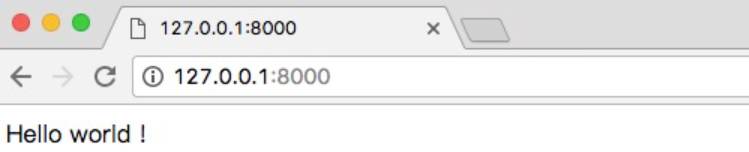
\includegraphics[width=0.4\textwidth]{part/互联/django/pic/概述/urlconf指向网站的根.png}
  \caption{urlconf指向网站的根}
  \label{fig:urlconf指向网站的根}
\end{figure}


  \item 适用于访问 \codeinline{/hello/} 路径
\begin{lstlisting}[style=demostyle,numbers=none]
$> cat HelloWorld/urls.py 
from django.urls import path
 
from . import views
 
urlpatterns = [
    path('hello/', views.hello),
]
\end{lstlisting}    
\begin{figure}[htpb]
  \centering
  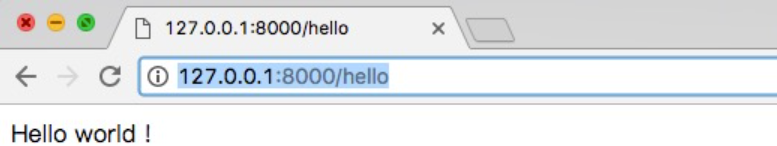
\includegraphics[width=0.4\textwidth]{part/互联/django/pic/概述/urlconf指向hello目录.png}
  \caption{urlconf指向hello目录}
  \label{fig:urlconf指向hello目录}
\end{figure}
  
\end{enumerate}
\end{example}

\section{路由视图过程}
\begin{enumerate}[label=\arabic*)]
    \item 在子应用\codeinline{TestModel}中的\codeinline{views.py}中定义一个\textcolor{YBXPurple}{视图函数}\codeinline{test\_view}，接收一个Web请求，返回一个Web响应。
    \item 在子应用\codeinline{TestModel}中的\textcolor{YBXPurple}{新建}一个\codeinline{urls.py}文件，定义一个\textcolor{YBXPurple}{路由}，将\codeinline{test\_view}与路由绑定。
\begin{lstlisting}[style=demostyle, numbers=none]
$> cat TestModel/urls.py
from django.urls import path
from .views import test_view

urlpatterns = [
    path('test/', test_view),
]
\end{lstlisting}    
    \item 在主应用\codeinline{mysite}中的\codeinline{urls.py}文件中，将子应用\codeinline{TestModel}的路由包含进来。
\begin{lstlisting}[style=demostyle, numbers=none]
from django.contrib import admin
from django.urls import path

from django.conf.urls import include, url

urlpatterns = [
    url(r"^", include('jobs.urls')), 
    path('admin/', admin.site.urls),  
    path('', include('TestModel.urls')),
]
\end{lstlisting}    
    \item 在浏览器中输入\codeinline{http://localhost:8000/test/}，即可看到如下页面：
\end{enumerate}

\begin{figure}[htpb]
    \centering
    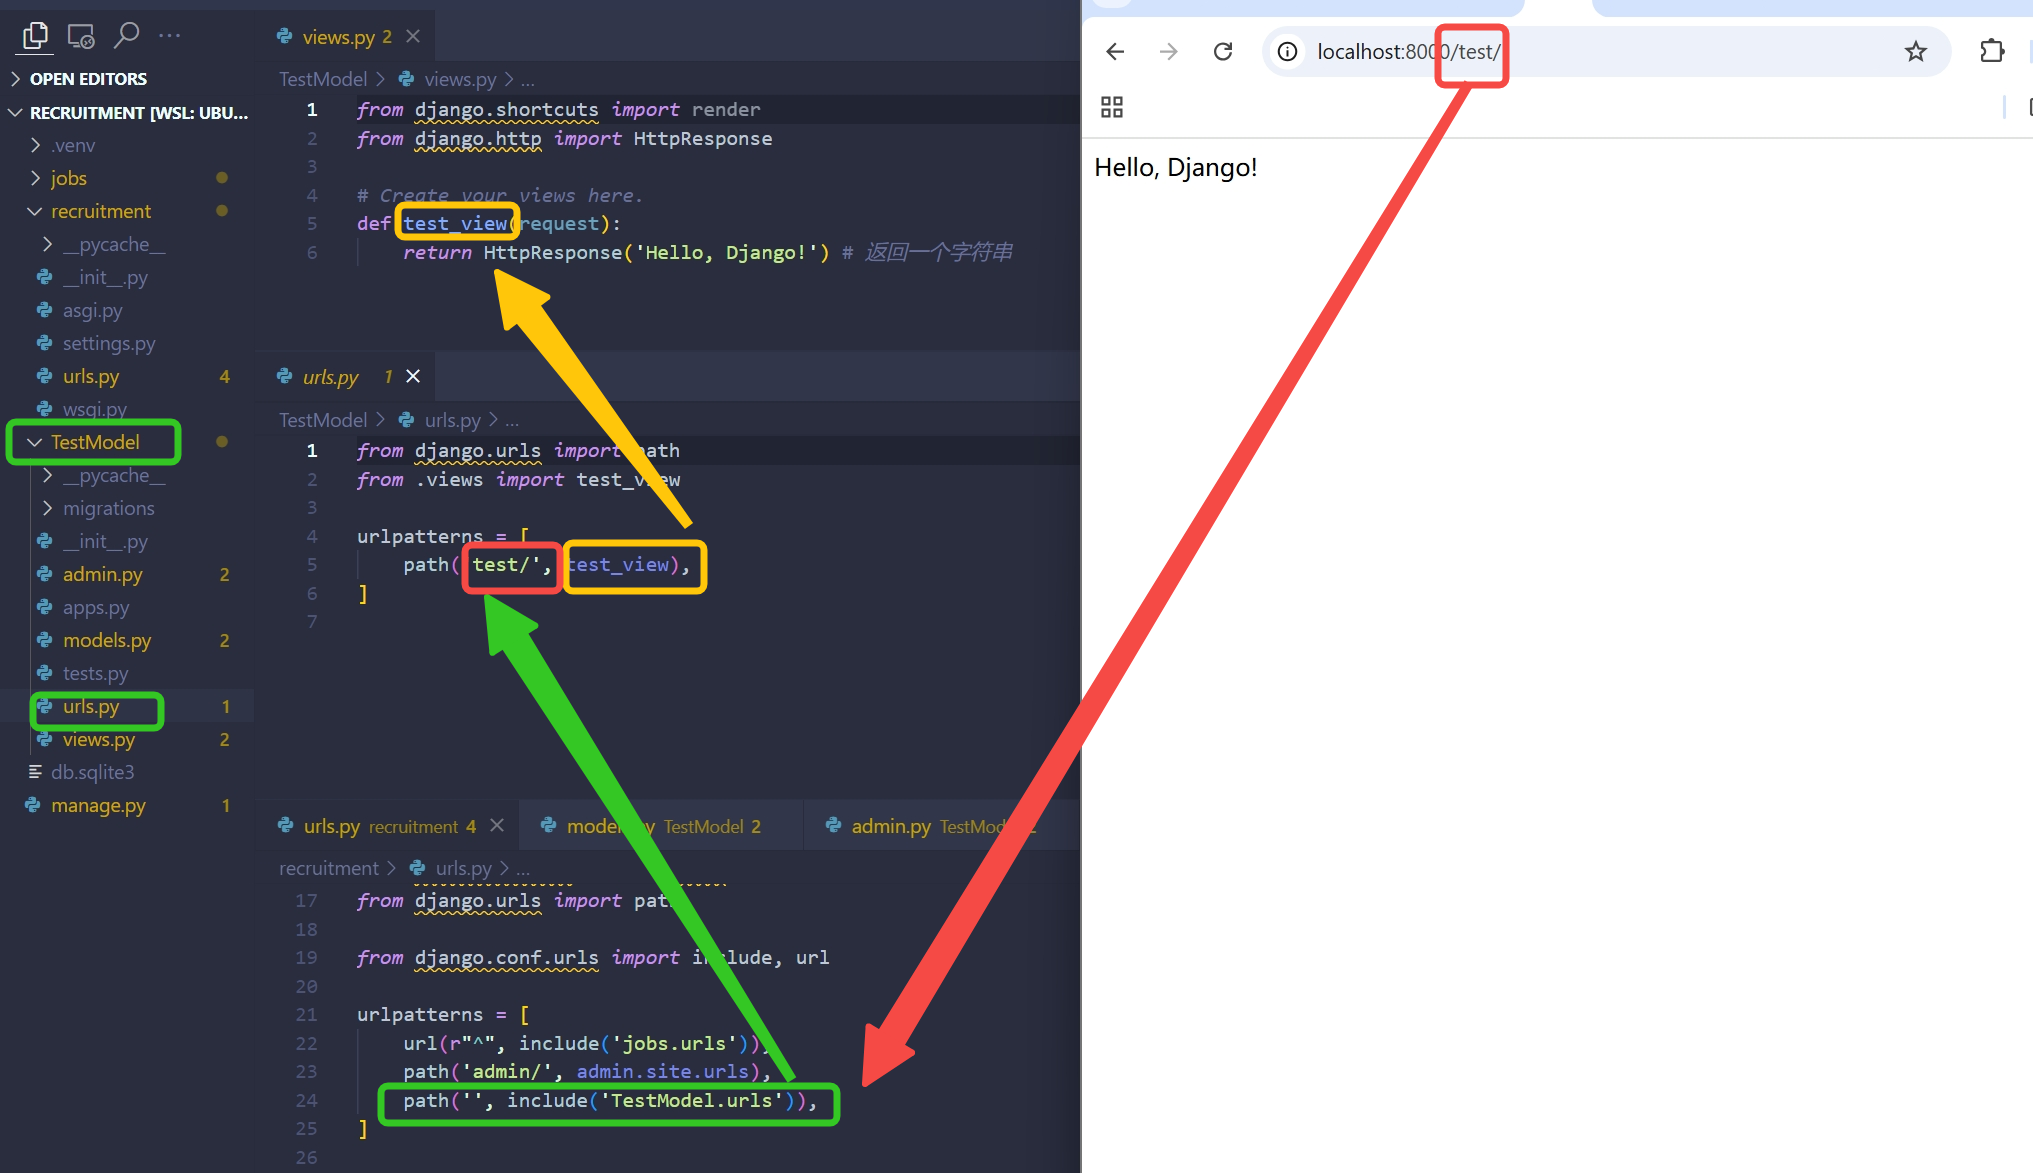
\includegraphics[width=0.6\textwidth]{part/互联/django/pic/视图/路由试图过程.png}
    \caption{路由视图过程}
    \label{fig:路由视图过程}
\end{figure}

其中路由的过程
\begin{enumerate}[label=\arabic*)]
    \item 用户在浏览器中输入\codeinline{http://localhost:8000/test/}。
    \item Django接收到请求，根据\codeinline{mysite/urls.py}中的路由配置，
    
    这里面是依次遍历\codeinline{jobs.urls}、\codeinline{admin}和\codeinline{TestModel.urls}。
    看这里面哪里个里面有\codeinline{test/}这个路由，找到了\codeinline{TestModel.urls}。

    \item 根据\codeinline{TestModel/urls.py}中的路由配置，找到了\codeinline{test\_view}。
    \item 调用\codeinline{test\_view}，返回一个\codeinline{HttpResponse}。
    \item 将\codeinline{HttpResponse}返回给浏览器。
\end{enumerate}







